\documentclass[10pt,a4paper]{article}
\usepackage[latin1]{inputenc}
\usepackage{amsmath}
\usepackage{amsfonts}
\usepackage{amssymb}
\usepackage{graphicx}
\usepackage{alltt}
\usepackage{color}
\usepackage{float}

\newcommand{\tbl}[1]{{\textcolor{blue}{#1}}}

\begin{document}
\begin{figure}[H]
\begin{center}
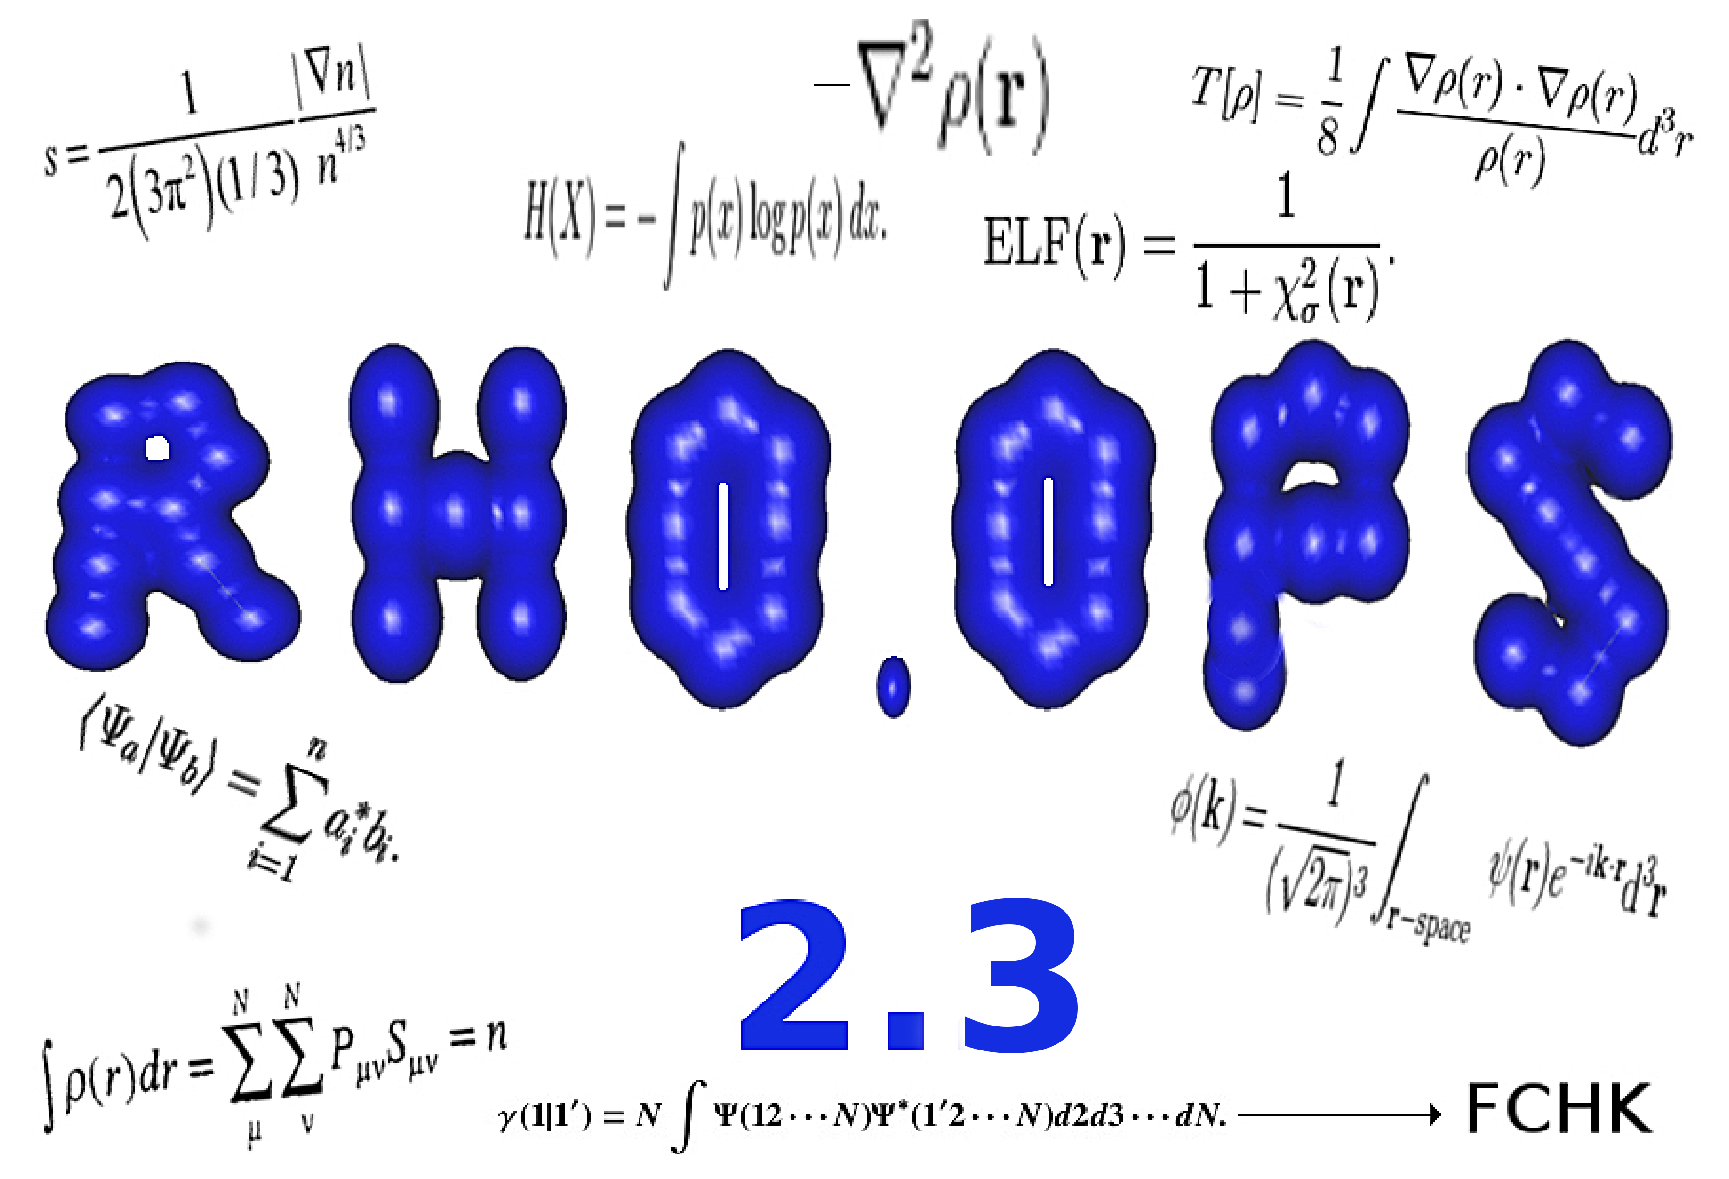
\includegraphics[angle=0, scale=0.5]{rhoops.eps}
\end{center}
\label{rhoops}
\end{figure}
\begin{center}
\begin{LARGE}
$\qquad$ Mauricio Rodr\'iguez Mayorga \newline
\end{LARGE}
{\color{white}a}\newline
$\qquad$ $\qquad$ \today
\end{center}

\section{\tbl{\textbf{How to cite the program}}}
Please if you are publishing the results obtained with RHO.OPS remember to cite correctly the program: \newline

   Rodr\'iguez-Mayorga, M.; RHO.OPS: Density Operations Program \& MO or NO Overalps Calculations; Donostia International Physics Center (DIPC), University of the Basque Country, Gipuzkoa, Donostia, Spain, 2015;\\ http://iqc.udg.es/$\sim$marm314/download/RHO\_OPS.2.3.tar.gz\newline

and please also cite the papers that deal with the most important features of the program:\newline

\noindent $\cdot$ Hahn. T.; Cuba - a library for multidimensional numerical integration. \textit{Comput. Phys. Commun.} 168, 78-95 (\textbf{2005}) DOI:10.1016/j.cpc.2005.01.010\newline
\noindent $\cdot$ Johnson S. G.; Cubature Package, http://ab-initio.mit.edu/cubature \newline
\noindent $\cdot$ Genz A. C. and Malik A. A.; An adaptive algorithm for numeric integration over an N-dimensional rectangular region. \textit{J. Comput. Appl. Math.} 6 (4), 295-302 (\textbf{1980}).\newline
\noindent $\cdot$ Berntsen J., Espelid. T. O., and Genz. A.; An adaptive algorithm for the approximate calculation of multiple integrals. \textit{ACM Trans. Math. Soft.} 17 (4), 437-451 (\textbf{1991}).\newline

\section{\tbl{\textbf{Compulsory keywords}}}

\noindent\$\textbf{NAME}. The name of the WFX, WFN or FCHK file.

\begin{verbatim}
   $NAME
   name.wfn, name.wfx or name.fchk
\end{verbatim}

\noindent For WFN files the multiplicity is compulsory information and there are two ways to pass it to the program. You can either use the \$\textbf{MULTIPLICITY} keyword or give the (Gaussian or Gamess) LOG file using the \$\textbf{LOG} keyword. See the following examples for more details: \newline

\noindent Using the multiplicity: \newline
\noindent \$\textbf{MULTIPLICITY}. The multiplicity of the calculation.

\begin{verbatim}
   $MULTIPLICITY
   (integer 1, 2, etc.)
\end{verbatim}

\noindent Using the LOG file: \newline
\noindent \$\textbf{LOG}. The multiplicity is read from the LOG file.

\begin{verbatim}
   $LOG
   name.log
\end{verbatim}

\noindent Also for WFN files and CAS calcultions, RHO.OPS requires that information by including the \$\textbf{CAS} keyword. This information is required to define the density type (i.e., relaxed or unrelaxed density). Include the Keyword:\newline
\begin{verbatim}
   $CAS
\end{verbatim}

\section{\tbl{\textbf{Optional keywords}}}

\noindent For open-shell correlated WFN files spin-dependent evaluations (separating alpha and beta contributions) are not computable. To ensure that the WFN is correct for those evaluations for the rest of cases (i.e., closed-shell and open-shell single determinat calculations $[$HF or DFT$]$  and closed-shell correlated calculations $[$MP2, CC, CI $]$) include if you want the \$\textbf{SPIN\_CALS} keyword.
\begin{verbatim}
   $SPIN_CALCS
\end{verbatim}
\noindent This keyword will test the WFN file and multiplicity. If the system is recognized to come from an open-shell correlated calculation, the spin-dependent evaluations are not allowed and the program will STOP at this stage. If the spin-dependent contributions are not required (e.g. total density evaluations, integral evaluations like Shannon Entropy in both spaces, scans of the densities in both spaces, etc.) DO NOT INCLUDE THE \$\textbf{SPIN\_CALS}  KEYWORD. IF THIS KEYWORD IS NOT INCLUDED, THE SPIN-DEPENTENT CONTRIBUTIONS FROM WFN FILES WILL BE SET TO ZERO.\newline  

\noindent For FCHK files, spin-dependent evaluations are always allowed. Nevertheless, NOs evaluations for FCHK files require the Atomic Overlap matrix  written by Gaussian in the LOG file if the Iop(3/33=4) is included in the Gaussian calculation. If NO evaluations are required, include the LOG file in the input using the \$\textbf{LOG} keyword.   

\begin{verbatim}
   $LOG
   name.log
\end{verbatim}

\noindent \$\textbf{BETA\_MOS}. Use the beta MO coefficients from the FCHK file. This keyword will only use them if they are available; If they are not, only the alpha will be use by RHO.OPS. With this keywords the MO are the odd numbered MOs. FCI calculations and CAS use only the alpha MOs then the even  and odd positions represent the same MO [i.e. MO number 1 and 2 will be the same for these methods but with different spin]. The use of ONLY alpha coefficients is set by default in RHO.OPS. Nevertheless, UCISD may use alpha and beta MOs for the expanssion then the \$\textbf{BETA\_MOS} keyword must be added to use BETA  orbitals.\newline

\noindent \$\textbf{DEBUG}. Debug-mode on. Provide some extra information to help locating errors. (Before contacting the developer include this keyword to get extra information about the possible error).\newline

\section{\tbl{\textbf{Evaluations keywords}}}

\noindent \$\textbf{PUNCTUAL\_R}. Punctual evaluations in position space are performed. These evaluations include gradients, laplacians and quantities used by local-hybrid Density Functional Theory (DFT) functionals. The input must be:\newline
\begin{verbatim}
   $PUNCTUAL_R
   (integer 1, 2, 3, etc) -> number of punctual evaluations 'n'
   (coordinates 1st point -> e.g. 0.0 0.0 0.0 
   .
   .                      -> Coordinates where the quantities are computed  
   .                         (as many as the integer given above 'n')
   (coordinates n-point) 
\end{verbatim}
\noindent \$\textbf{PUNCTUAL\_P}. Punctual evaluations in momentum space are performed. These evaluations include gradients and laplacians. The input must be:\newline
\begin{verbatim}
   $PUNCTUAL_P
   (integer 1, 2, 3, etc) -> number of punctual evaluations 'n'
   (coordinates 1st point -> e.g. 0.0 0.0 0.0 
   .
   .                      -> Coordinates where the quantities are computed  
   .                         (as many as the integer given above 'n')
   (coordinates n-point) 
\end{verbatim}
\noindent \$\textbf{SCAN\_R}. Scan the density in position space, the norm of the gradient and the laplacian. These evaluations are usefull for gnuplot plots of the density along some direction:\newline
\begin{verbatim}
   $SCAN_R
   (initial coordinates)  -> example 0.0 0.0 0.0
   (integer total number of points)
   step_size              -> example 0.01
   direction              -> example z (can be x, y or z)
\end{verbatim}
\noindent \$\textbf{SCAN\_P}. Scan the density in momentum space, the norm of the gradient and the laplacian. These evaluations are usefull for gnuplot plots of the density along some direction:\newline
\begin{verbatim}
   $SCAN_P
   (initial coordinates)  -> example 0.0 0.0 0.0
   (integer total number of points)
   step_size              -> example 0.01
   direction              -> example z (can be x, y or z which refer to px, py or pz)
\end{verbatim}
\noindent \$\textbf{SCAN\_ELF}. Scan the density, the norm of the gradient and ELF [JCP {\bf 92}, 5397 (1990)]. These evaluations are usefull for gnuplot plots of the density or the ELF along some direction:\newline
\begin{verbatim}
   $SCAN_ELF
   (initial coordinates)  -> example 0.0 0.0 0.0
   (integer total number of points)
   step_size              -> example 0.01
   direction              -> example z (can be x, y or z)
\end{verbatim}
\noindent \$\textbf{SCAN\_INDICATORS}. Scan the density, ID\_alpha, ID\_beta, IND\_alpha and IND\_beta. These evaluations are usefull for gnuplot plots of the density or the INDICATORS along some direction:\newline
\begin{verbatim}
   $SCAN_INDICATORS
   (initial coordinates)  -> example 0.0 0.0 0.0
   (integer total number of points)
   step_size              -> example 0.01
   direction              -> example z (can be x, y or z)
\end{verbatim}
This is only available for FCHK files $[$including the LOG file computed with Iop(3/33=4)$]$, WFX files and WFN files.\newline 
\noindent \$\textbf{DMN\_R}. This keyword must be use for linking FCHK files (which contain the coefficients for the MOs) with unformatted DMN files obtained with DMN Program of Dr. E. Matito. This keyword allows evaluation of the trace of the corresponding DMN and also perform punctual evaluations in position space of those DMN matrices (density and gradient at the coalescence point $1=1$'). Actually, only up to DM1 files are supported at the moment. 
\begin{verbatim}
   $DMN_R
   1              -> Include this flag
   name.dm1       -> name of the DMX file
   1              -> order of name.dmX
   coord. 1       -> (e.g. 0.0 0.0 0.0)
   coord. 1'      -> (e.g. 0.2 0.4 3.4532)
\end{verbatim}
For DM1 calculations with ${\bf r} ={\bf r}$' (which is the coalescence point) the density, the norm of the gradient and the components of the gradient of the density will also be computed by default. Also for DM1 files, the occupation of the NOs in position space is printed (The NOs are available but not used by this keyword).
\newline
\newline
\noindent \$\textbf{DMN\_P}. This keyword must be use for linking FCHK files (which contain the coefficients for the Molecular Orbitals in the momentum space (MOps) $[$the MOps are obtained using a Fourier transform of the MOs$]$) with unformatted DMN files obtained with DMN Program of Dr. E. Matito. This keyword evaluates the trace of the corresponding DMN and also performs punctual evaluations of those DMN matrices (density and gradients at the coalescence point $1=1$'). Actually, only up to DM1 files are supported at the moment.
\begin{verbatim}
   $DMN_P
   1              -> Include this flag
   name.dm1       -> name of the DMX file
   1              -> order of name.dmX
   coord. 1       -> (e.g. 0.0 0.0 0.0)
   coord. 1'      -> (e.g. 0.2 0.4 3.4532)
\end{verbatim}
For DM1 calculations with ${\bf p} ={\bf p}$' (which is the coalescence point) the density, the norm of the gradient and the components of the gradient of the density will also be computed by default. Also for DM1 files, the occupation of the NOs in momentum space is printed (The NOs are available but not used by this keyword). 
\newline
\newline
\noindent \$\textbf{CPS}. This option calls for the calculation of critical points (Bond Critical Points, Ring Critical Points and Cage Critical Points).\newline
\begin{verbatim}
   $CPS
\end{verbatim}
\section{\tbl{\textbf{Indicators}}}
\noindent \$\textbf{INDICATORS}. This option calls for the calculation of correlation indicators (I2(n$_i$), ID(n$_i$), IND(n$_i$), ID(n$_i$)$+$IND(n$_i$) and S(n$_i$)). Be aware that for open-shell correlated WFN files (where we have spin summed NOs) and for FCHK files computed without the LOG file (when we do not have the AOs overlap) these quantities will not be computed. Include the keyword \$\textbf{INDICATORS} for these evaluations: \newline
\begin{verbatim}
   $INDICATORS
\end{verbatim}
\noindent \$\textbf{INDICATORS\_DMN}. This keyword allows to calculate the correlation indicators (I2, ID, IND, IT and S(ni)) using DM1 files with their corresponding FCHK files declared in the \$\textbf{NAME} statement.\newline The \$\textbf{INDICATORS} keyword must be followed by this new keyword:
\begin{verbatim}
   $INDICATORS
   $INDICATORS_DMN
   name.dm1         -> name of the DM1 file
\end{verbatim}
\noindent Be aware that if the \$\textbf{INTEGRALS\_DMN} keyword is used and the \newline\$\textbf{INDICATORS\_DMN} is used too. THE DM1 FILE MUST BE THE SAME FOR BOTH!   
\newline
\newline
\section{\tbl{\textbf{Integrals of the density}}}
\noindent \$\textbf{INTEGRALS}. This option allows the calculation of several quantities that require integration (Density in Position Space $[$density$]$, Square of the density in Position Space $<\rho>$ $[$rho$]$ (Not available for FCHK+DM1 files!), Density in Momentum Space $[$densityp$]$, Shannon entropy in both spaces $[$shannon or shannonp$]$, Fisher Integral in both spaces $[$fisher or fisherp$]$, Inertia Tensors in both spaces $[$inertia or inertiap$]$, Thomas-Fermi Kinetic Energy $[$ttf$]$, Weiszacker Kinetic Energy $[$tw$]$, Shannon Entropy Powers of the corresponding Shannon Entropies, Fisher-Shannon products, $<r>$ $[$r1$]$, $<r^2>$ $[$r2$]$, $<r^{-1}>$ $[$rm1$]$, $<p>$ $[$p1$]$, $<p^2>$ $[$p2$]$, dipolar moment $[$dipolar$]$ (except for cubature), quadrupole moments $[$quadrupole$]$ (not available for cubature), MOs overlaps for FCHK files, single-determinat WFX files and single-determinat WFN files (HF and DFT) and NOs overlaps for all WFX, WFN files and for FCHK files computed with the LOG file $[$sij$]$), $[$r1\_moment$]= \int \phi _i({\bf r}) \phi _j ({\bf r}) {\bf r} d {\bf r}$ matrix (only avaliable for Quadrature and mainly for atoms). Two libraries and a quadrature rule are available. The two libraries are CUBA (which includes four different procedures Cuhre$[$deterministic$]$, Vegas, Suave and Divonne $[$Montecarlo$]$) and CUBATURE $[$deterministic$]$.\newline
The Quadrature rule (Lebedev for unit sphere and Legendre for radial) is recommended for all momentum space evaluations and for atoms or small systems in position space.\newline
Cuba library is the fastest one for all spaces and only if the precision is not achieved other procedure must be chosen (sometimes is better to use Quadrature for momentum space or really small systems like atoms). Cuba was developed for vectorial evaluations over the grid points using a well paralelized code. Increasing the number of cores may lead to ultrafast results. Among all Cuba procedures, Cuhre is strongly recommended since it is deterministic but may fail when the important points for the evaluations lie far from the axis defined. If the important points lie far from the axis, Montecarlo procedures would avoid this issue and the user may preffer to chose a Montecarlo procedure eventhough there might be a loss of precision (Max. Prec. Montecarlo $\approx 1e^{-4}$). By the nature of Cuba library, all quantities will be evaluated at once for each space (e.g. the Density, Thomas-Fermi Kinetic Energy, Shannon Entropy, Shannon Entropy Power, etc. Will only require one evaluation of the electronic position space density for each point of the grid) In the case of overlaps, for WFN files the entire Sij matrix is calculated at once whereas for FCHK files, only an entire column of the Sij matrix is performed at once. \newline
Cubature is a good option when only one quantity is required (e.g. only position space Shannon). The calculation of Inertia Tensors is then not implemented for this procedure since it requires more than one evaluation at once. For Sij overlaps, the TWO MO or NO involved in the overlap must be defined as described bellow. Use Cubature with caution since the limit for the maximum number of evaluationsis very large by default and for some cases might seem to be infite! (Cubature is not paralellized so it may take a while to get the final results for some systems). \newline
Cubature2 is a OMP parallelized, by me, version of Cubature. It will work for FCHK, WFX and WFN files but not for DM1$+$FCHK files (in this later case, compute the FCI FCHK file and work with it). The calculation of Inertia Tensors is not implemented for this procedure neither Sij overlaps. Again, have caution when working with Cubature2 since the limit for the maximum number of evaluationsis very large by default and for some cases might seem to be infite time!\newline
All integrals are performed in spherical coordinates system and the information about the intervals for the radial coordinate, polar angle and azimuthal angle must be given in the input. Please, notice that once an interval is defined it will be FIXED for ALL integrals of Cuba and Cubature. The only exception which will not keep fixed intervals is the Sij matrix calculation using Cuba library (see bellow). On the other hand, Quadrature will always allow to define an interval for each calculation (e.g. Density and Shannon may have different intervals). Only for the Inertia Tensors interval will be fixed to calculate the position of the center of electronic charge (RCC), the Inertia Tensor of the center of electronic charge (Im) and the Inertia Tensor at the center of electronic charge (IM). In general, Inertia Tensors are always given AT THE CENTER OF ELECTRONIC CHARGE!\newline  
\newline
\noindent CUBA example:\newline
\begin{verbatim}
   $INTEGRALS
   cuba
   ncores               -> Number of cores to be used by cuba library (1 to idle cores) 
   error_abs error_rel    
   min_evals max_evals  -> Minimum and maximum number of evaluations (e.g. 0 1000000)
   operations           -> Total number of integrals to cumpute N (integer)
   operation_1          -> (density, densityp, ..., etc.) 
   operation_2          -> (density, densityp, ..., etc.) 
   .
   .
   .
   .
   .
   operation_N          -> (density, densityp, ..., etc.) 
   procedure            -> (cuhre, vegas suave or divonne)
   r_min  r_max         -> radial coord. limits (e.g. 0 1.0e99)
   t_min  t_max         -> polar coord. limits  (e.g. 0 180)
   phi_min phi_max      -> azimuthal coord. limits (e.g. -180 180)
\end{verbatim}
{\color{white} xxx \newline}
\noindent CUBATURE example:\newline

\begin{verbatim}
   $INTEGRALS
   cubature
   error_abs            -> Abs. error in accuracy.     
   operations           -> Total number of integrals to cumpute N (integer)
   operation_1          -> (density, densityp, ..., etc.) 
   operation_2          -> (density, densityp, ..., etc.) 
   .
   .
   .
   .
   .
   operation_N          -> (density, densityp, ..., etc.) 
   r_min  r_max         -> radial coord. limits (e.g. 0 1.0e99)
   t_min  t_max         -> polar coord. limits  (e.g. 0 180)
   phi_min phi_max      -> azimuthal coord. limits (e.g. -180 180)
\end{verbatim}
{\color{white} xxx \newline}
\noindent CUBATURE2 example:\newline

\begin{verbatim}
   $INTEGRALS
   cubature2
   error_abs            -> Abs. error in accuracy.     
   operations           -> Total number of integrals to cumpute N (integer)
   operation_1          -> (density, densityp, ..., etc.) 
   operation_2          -> (density, densityp, ..., etc.) 
   .
   .
   .
   .
   .
   operation_N          -> (density, densityp, ..., etc.) 
   r_min  r_max         -> radial coord. limits (e.g. 0 1.0e99)
   t_min  t_max         -> polar coord. limits  (e.g. 0 180)
   phi_min phi_max      -> azimuthal coord. limits (e.g. -180 180)
\end{verbatim}
\noindent QUADRATURE example:\newline
\begin{verbatim}
   $INTEGRALS
   quadrature
   rad ang              -> rad=total radial points & ang=total ang points in the sphere.     
   operations           -> Total number of integrals to cumpute N (integer)
   operation_1          -> (density, densityp, ..., etc.) 
   r_min  r_max         -> radial coord. limits (e.g. 0 1.0e99)
   t_min  t_max         -> polar coord. limits  (e.g. 0 180)
   phi_min phi_max      -> azimuthal coord. limits (e.g. -180 180)
   operation_2          -> (density, densityp, ..., etc.) 
   r_min  r_max         -> radial coord. limits (e.g. 0 1.0e99)
   t_min  t_max         -> polar coord. limits  (e.g. 0 180)
   phi_min phi_max      -> azimuthal coord. limits (e.g. -180 180)
   .
   .
   .
   .
   .
   operation_N          -> (density, densityp, ..., etc.) 
   r_min  r_max         -> radial coord. limits (e.g. 0 1.0e99)
   t_min  t_max         -> polar coord. limits  (e.g. 0 180)
   phi_min phi_max      -> azimuthal coord. limits (e.g. -180 180)
\end{verbatim}

\noindent Note 1: The estimated error of CUBA is equal to the max(Eabs,Erel$|$Integration$|$). The absolute error in the accuracy of the integration recommended for instance is $1e^{-4}$ with a relative error in the accuracy $1e^{-3}$. Be aware that increasing their values may require more evaluations. Also notice that CUBATURE only has the maximum error as input parameter and there is no maximum number of evaluations. This fact may cause that the integration procedure be kept running for very long periods of time if the requested accuracy is not reached!\newline
\newline
\noindent Note 2: Sij operation requires extra information (compulsory information).  \newline   

\noindent CUBA (Sij is not compatible with other evaluations i.e. Shannon, Shannonp, etc.): \newline
\begin{alltt}
   $INTEGRALS
   cuba
   .      
   .
   .
   sij               -> operation
   NO or MO          -> Use NO or MO
   nregions          -> Number of regions N (integer)
   procedure         -> (cuhre, vegas suave or divonne)
   r\_min  r\_max       -> radial coord. limits (e.g. 0 1.0e99)
   t\_min  t\_max       -> polar coord. limits  (e.g. 0 180)       ==> Region 1
   phi\_min phi\_max    -> azimuthal coord. limits (e.g. -180 180)
   r\_min  r\_max       -> radial coord. limits (e.g. 0 1.0e99)
   t\_min  t\_max       -> polar coord. limits  (e.g. 0 180)       ==> Region 2
   phi\_min phi\_max    -> azimuthal coord. limits (e.g. -180 180)
   .
   .  
   r\_min  r\_max       -> radial coord. limits (e.g. 0 1.0e99)
   t\_min  t\_max       -> polar coord. limits  (e.g. 0 180)       ==> Region N
   phi\_min phi\_max    -> azimuthal coord. limits (e.g. -180 180)
\end{alltt}
\noindent CUBATURE (the two MO or NO involved must be specified): \newline
\begin{alltt}
   $INTEGRALS
   cubature
   .      
   .
   .
   sij                -> operation
   NO or MO           -> Use NO or MO
   Orb1 Orb2          -> Orbitals involved (e.g. 1 3) 
   r\_min  r\_max       -> radial coord. limits (e.g. 0 1.0e99)
   t\_min  t\_max       -> polar coord. limits  (e.g. 0 180)
   phi\_min phi\_max    -> azimuthal coord. limits (e.g. -180 180)
   .
   .  
\end{alltt}
\noindent QUADRATURE: \newline
\begin{alltt}
   $INTEGRALS
   quadrature
   .
   .
   .
   sij                 -> operation
   r\_min  r\_max         -> radial coord. limits (e.g. 0 1.0e99)
   t\_min  t\_max         -> polar coord. limits  (e.g. 0 180)
   phi\_min phi\_max      -> azimuthal coord. limits (e.g. -180 0)
   NO or MO            -> Use NO or MO
   sij                 -> operation 
   r\_min2  r\_max2       -> radial coord. limits (e.g. 0 1.0e99)
   t\_min2  t\_max2       -> polar coord. limits  (e.g. 0 180)
   phi\_min2 phi\_max2    -> azimuthal coord. limits (e.g. 0 180)
   NO or MO            -> Use NO or MO
   .
   .
\end{alltt}
Note 3.1: The int file 1 is assigned by Cuba and Quadrature to the first interval, the rest of intervals will lead to more int files which will be numbered according the order in which they appear in the input file. For WFN and WFX files MOs are not available, unless they come from a single determinant calculation, where the MOs are equal to the NOs so this keyword can be set to MO or NO. For correlated calculations the MOs are not availabe in WFN and WFX files and MO will be set to NO. On the other hand, MOs are always available for FCHK files but NOs are available only if the LOG file has been included (the LOG file must containg the Atomic Overlap matrix computed with the iop(3/33=4) as it was mentioned before).    
\newline
Note 3.2: The Quadrature procedure allows to calculate all n-regions at the same time. As an example, since the regions are named according to the order in which they are enumerated. In the above example region 1 corresponds to $-180 <\phi \leq 0$ and region 2 corresponds to $0 <\phi \leq 180$. \newline
\newline
\newline
\noindent \$\textbf{INTEGRALS\_DMN}. This keyword allows to perform the integrals defined in the \$\textbf{INTEGRALS} section (including overlaps $[$sij$]$ when NOs built using the DM1 matrix are required). Notice that \$\textbf{DMN\_R} and \$\textbf{DMN\_P} keywords are not required to this end and the name of the DMI matrix will not be read from them. Also notice that all the integrals will be computed using DM1 files plus FCHK files in both spaces (position and momentum). Be aware that the densities and the gradients of the density are calculated reading the DM1 matrix `on the fly' for each evaluation so the execution time may increase easily for larg DM1 files! If the DM1 file is storable, include the \${\textbf{DMNINCORE} keyword and store it because the reading time will be avoided and the procedure will go faster. Finally, it is strongly recommended to write the new FCI FCHK file (see bellow how). Because the Total Density stored there in AOs would lead to even faster evaluations of the density than using MOs and the DM1 matrix (see bellow how to obtain a FCHK FCI file). 
\begin{verbatim}
   $INTEGRALS_DMN
   name.dm1
\end{verbatim}
{\color{white} x}
\newline
\newline 
\noindent \$\textbf{DMN\_THRESHOLD}. By default, the terms from the DMN are used for trace, integrals, evaluations, etc. Only if their absolute value is greater or equal to $1e^{-8}$. To define a new threshold, you must include this keyword. Be aware that ALL evaluations including the DMN files will be computed with this threshold.
\begin{verbatim}
   $DMN_THRESHOLD
   number         -> e.g. 1.0e-6
\end{verbatim} 
\section{\tbl{\textbf{Intracule}}}
\noindent \$\textbf{INTRACULE}. This option allows for the evaluation of the Intracule density.\newline
\begin{verbatim}
   $INTRACULE
    name_file.dm2        -> Name of the DM2 file
    x12   y12  z12       -> Intracule point to evaluate 
    ncores               -> Number of cores to be used by cuba library
    error_abs error_rel    
    min_evals max_evals  -> Minimum and maximum number of evaluations (e.g. 0 1000000)
    procedure            -> (i.e. Cuhre, Vegas, etc.)
\end{verbatim}
This calcualation needs the DM2 in core so include the \$\textbf{DMNINCORE} keyword.
\section{\tbl{\textbf{Total Position Spread}}}
\noindent RHO.OPS has the option to calculate the Total Position Spread $[$TPS$]$ (see: $https://en.wikipedia.org/wiki/Total\_position\_spread$) for more details. The TPS calculated is first the approximated TPS (compute using only the density) but if the moments $<x1x2>$, $<x1y2>$, $<x1z2>$, $<y1y2>$, $<y1z2>$ and $<z1z2>$ are given, the exact TPS is also computed. Only CUBA procedure is available for this quantity. 
\begin{verbatim}
   $TPS
   ncores               -> Number of cores to be used by cuba library (1 to idle cores) 
   error_abs error_rel    
   min_evals max_evals  -> Minimum and maximum number of evaluations (e.g. 0 1000000)
   procedure            -> (i.e. Cuhre, Vegas, etc.)
   DM2 moments          -> (<x1x2>, <x1y2>, <x1z2>, <y1y2>, <y1z2> and <z1z2>)
\end{verbatim}
Note: Set the moments  ($<x1x2>$, $<x1y2>$, $<x1z2>$, $<y1y2>$, $<y1z2>$ and $<z1z2>$) to zero if only the approximated TPS is needed.\\
Note2: The DM2 moments  ($<x1x2>$, $<x1y2>$, $<x1z2>$, $<y1y2>$, $<y1z2>$ and $<z1z2>$) can be computed using RHO2\_OPS code (RHO2\_OPS also computs the TPS and all computations are analytic using the DM2 in primitives). \\
Note3: If DM2 moments  are used, recall to use a FCHK, WFX or WFN file whose density is the one corresponding to the DM2 (i.e. check if a DM1 FCHK/WFN/WFX file is needed).  
\section{\tbl{\textbf{Density similarity indexes}}}
\noindent RHO.OPS can compute some density similarity indexes $[$DENS\_SIM$]$ (see Sheila's thesis for more details). Only CUBA procedure is available for this calculation. Two FCHK or WFN files will be stored. 
\begin{verbatim}
   $DENS_SIM
   second_fchk          -> Name of the second FCHK or WFN file. 
   ncores               -> Number of cores to be used by cuba library (1 to idle cores) 
   error_abs error_rel    
   min_evals max_evals  -> Minimum and maximum number of evaluations (e.g. 0 1000000)
   procedure            -> (i.e. Cuhre, Vegas, etc.)
   density or nuclei    -> (use $\rho ({\bf r})$ or the nuclei for the orientation)
   only or gradient     -> (simmilarity 'only' (density) or 'gradient' also gradient)
\end{verbatim}
Note: Notice that WFN and FCHK files can be used at the same time.\\
\section{\tbl{\textbf{Integrated polarizability and hyperpolarizability}}}
\noindent RHO.OPS can compute polarizabilities and hyperpolarizabilities. Only CUBA procedure is available for this calculation. Five FCHK or WFN or WFX files will be stored (the one in \$NAME is the without field one). 
\begin{verbatim}
   $INT_POL_HYPERPOL
   second_fchk          -> Name of the second FCHK or WFN file (- F). 
   third_fchk           -> Name of the second FCHK or WFN file (  F). 
   fourth_fchk          -> Name of the second FCHK or WFN file (-2F). 
   fifth_fchk           -> Name of the second FCHK or WFN file ( 2F). 
   ncores               -> Number of cores to be used by cuba library (1 to idle cores) 
   error_abs error_rel    
   min_evals max_evals  -> Minimum and maximum number of evaluations (e.g. 0 1000000)
   procedure            -> (i.e. Cuhre, Vegas, etc.)
   field                -> F
   direction            -> x, y or z.  
\end{verbatim}
Note: Notice that WFN and FCHK files can be used at the same time.\\
\section{\tbl{\textbf{Plots}}}
\noindent RHO.OPS has the option to plot the density, Shannon entropy and Fisher Integral for position and momentum space. To do so, RHO.OPS calls {\tbl{\textbf{gnuplot}}}. There are two ways to call gnuplot. Either writing the explicit PATH or using NO PATH (if "gnuplot" command already works on your terminal). Two types of plots are available: 2D plots and 3D plots (but they are mutually exclusive). Here we have a couple of examples of usage:
\newline
\newline
\noindent 2D: \newline
\begin{verbatim}
   $PLOT
   PATH           -> Write the path to gnuplot or NO PATH.
   2D                (e.g. NO PATH).
   axis           -> character (x, y or z).
   min   max      -> interval to scan (e.g. -3 3)
   steps width    -> real number (e.g. 0.01)
   N              -> number of plots to perform (integer e.g. 3)
   operation1     -> e.g. density
   operation2     -> e.g. shannon
   .
   .
   operationN     -> e.g. shannonp
   extra_lines    -> integer (e.g. 0 or j)
   extra_command1 -> added extra command to gnuplot (e.g. reset)
   .
   .
   .
   extra_commandj
\end{verbatim}
Note 1: In position space use: density, shannon or fisher; in momentum space use densityp, shannonp or fisherp. \newline
Note 2: Notice that if {\tt extra\_lines$=0$}, no extra commands will be used apart from the default ones. To see the default ones, check the files .plot2 \newline
Note 3: Local Hybrid quantities like $\tau _W (r)/\tau (r)$ data files might be generated using local\_hybrids as an operation. Notice that using this operation will make shannon, etc. Be not computed. The data files are generated but the .plot2 file and .eps is only computed for the density but the user might use that .plot2 file as template to plot the rest of files.\newline  
\newline  
\noindent 3D: \newline
\begin{verbatim}
   $PLOT
   PATH           -> Write the path to gnuplot or NO PATH.
   3D                (e.g. NO PATH).
   axis1 axis2    -> two characters (x y, x z, z y, y z, etc).
   min1   max1    -> interval for first axis (e.g. -3 3)
   min2   max2    -> interval for second axis (e.g. -4 4)
   steps widths   -> real numbers (e.g. 0.01 0.5)
   Axis Fixed_Num -> Axis is the axis not scanned (e.g. z) and Fixed_Num the fixed value.  
   N              -> number of plots to perform (integer e.g. 3)
   operation1     -> e.g. density
   operation2     -> e.g. shannon
   .
   .
   operationN     -> e.g. shannonp
   extra_lines    -> integer (e.g. 0 or j)
   extra_command1 -> added extra command to gnuplot (e.g. reset)
   .
   .
   .
   extra_commandj
\end{verbatim}
Note 1: In position space use: density, shannon or fisher; in momentum space use densityp, shannonp or fisherp. \newline
Note 2: Notice that if {\tt extra\_lines$=0$}, no extra commands will be used apart from the default ones. To see the default ones, check the files .plot3 \newline
Note 3: The fixed axis is the one not changed i.e., if you decide to scan x and y componets, the fixed one must be z. The {\tt Fixed\_Num} may be 0 to scan in the plane (x, y, 0).\newline 
Note 4: Local Hybrid quantities like $\tau _W (r)/\tau (r)$ data files might be generated using local\_hybrids as an operation. Notice that using this operation will make shannon, etc. Be not computed. The data files are generated but the .plot3 file and .eps is only computed for the density but the user might use that .plot3 file as template to plot the rest of files.\newline  
\newline
\newline 
\noindent \$\textbf{PLOTS\_DMN}. Use this keyword plus the name of the DM1 file to evaluate densities, Shannon entropies and Fisher Integrals using DMN results.\newline 
\begin{verbatim}
   $Plots_DMN
   name.dm1
\end{verbatim}
\section{\tbl{\textbf{DMN IN CORE}}}
\noindent \$\textbf{DMNINCORE}. Use this keyword plus the amount of ram memory, in Gb, to evaluate using the DM1 matrix in core. Be aware that position space and momentum space evaluations will not use the same stored DM1 matrices (one DM1 matrix is stored for each space for Quadrature and Plots), Cuba also stores one DM1 for each space and finally, Cubature integrations will store one DM1 matrix for each integration asked (even in the same space!)\newline 
\begin{verbatim}
   $DMNINCORE
   number -> Ram in Gb
\end{verbatim}
\section{\tbl{\textbf{PSEUDO WFX FILES}}}
\noindent \$\textbf{WFX\_PRINT}. This keyword will print a pseudo wfx file (in alpha and beta components separated if it is possible). It will print only the number of orbitals and the occupations as it is needed for ESI. For FCHK files we need the LOG file, computed with keyword Iop(3/33=4), as it was commented before (see keyword \$\textbf{LOG} for more details). For WFX, WFN files, the number of NOs and the occupations are read and copied directly to the pseudo wfx files.   
\begin{verbatim}
   $WFX_PRINT
\end{verbatim}
If the DM1 file is available, include:
\begin{verbatim}
   $WFX_PRINT_DMN
   name.dm1
\end{verbatim}
And the DM1 matrix will be diagonalized with the alpha and beta components separated ALWAYS. The occupations and the number of orbitals printed in the wfx files will be the size of the alpha$+$beta basis (simply sum the odd and even occupations for close shell systems).   
\section{\tbl{\textbf{DM1 FCHK FILES}}}
\noindent \$\textbf{FCHK\_DM1}. This keyword requires the \$\textbf{DMNINCORE} keyword (see the \$\textbf{DMNINCORE} for more details). It will create a FCHK file where the Total Density and Spin Density (if it is an open-shell system) will be computed using the DM1 file from DMN making it a DM1 FCHK file. This keyword also requires the name of the DM1 file in the input. For CAS FCHK files whose Total Density comes from a state average calculation, the Total Density is that of the highest state and the DM1 file is needed to rebuild a FCHK file for the state of interest. Include the keyword \$\textbf{CAS} in this case!    
\begin{verbatim}
   $FCHK_DM1
   name.dm1
\end{verbatim}
Note that if Beta MO coefficients and Beta MO energies are present, the word Beta is rewriten using capital letters and replacing E for 3 (Beta $\rightarrow$B3TA).
\section{\tbl{\textbf{Transformation of int files}}}
\noindent RHO.OPS int files generated using the \$\textbf{INTEGRALS} command, with sij, are written is Gaussian AO Overlap matrices format $[$the ones obtained using  IOP(3/33=4)$]$. Which means that the lower diagonal part of the overlap matrix generated by RHO.OPS is written using columns of the MO or NO overlap matrix (Up to five columns. If there are more than five columns in the MO or NO Overlap Matrix, the next five ones are written bellow and so on). Whereas ESI-3c program of Dr. E. Matito requires int files written in rows. RHO.OPS is able to transform the name\_Xn.int file into a Transform\_name\_Xn.int file written in columns. To do so, include the keyword \$\textbf{ESI\_INT} when calculating int files. See the example bellow:
\begin{verbatim}
   $ESI_INT
   region         -> Integer (e.g. 1, 2, etc.)
\end{verbatim}
\noindent Note. Only the compulsory keywords(\$\textbf{NAME} $[$FCHK, WFX or WFN$]$ and \$\textbf{LOG} or \$\textbf{MULTIPLICITY} $[$for WFN files$]$) plus this NEW keyword are needed to create transformed int files from previously created int files. The FCHK, WFN or WFX file must be the same as the one used for the MO or NO overlaps calculation because the size of the basis is read from them!
\section{\tbl{\textbf{Cube file}}}
\noindent RHO.OPS cube files generated using the \$\textbf{CUBE} command. Only FCHK, WFX and WFN are available. For ELF $[$elfa or elfb$]$, INDICATORS and NOs using FCHK files, again the LOG file is needed $[$the ones obtained using  IOP(3/33=4)$]$. The properties available are the densities $[$density or densityp$]$, Laplacians $\nabla ^2 \rho(r)$ or $-\nabla ^2 \rho(r)$  [laplacian or nlaplacian], Shannon entropies $[$shannon or shannonp$]$, Fisher integrals $[$fisher or fisherp$]$, ELF (all, alpha and beta $[$ELF, ELFa and ELFb$]$), ID $[$id$]$, IND $[$ind$]$, ID\_alpha $[$ida$]$, ID\_beta $[$idb$]$, IND\_alpha $[$inda$]$, ID\_beta $[$indb$]$, I\_Total $[$idnd$]$, MOs and NOs. See the example bellow:
\begin{verbatim}
 $CUBE
 operation -> density, densityp, shannon, shannonp, etc.
 nx ny nz  -> number of points for each axis x, y or z (e.g. 40 40 40)
 stepx stepy stepz -> step size for the cube file (e.g 0.283459 0.283459 0.283459)
 orbital   -> only for `mo' or `no' include an extra line with the orbital to use
                for the evalutations (e.g. 1). 
\end{verbatim}
\noindent Note1: If you open the CUBE file with Gabedit Program, use Gaussian Laplacian to analize the plots. 
\noindent Note2: The number of points times the step would give a whole size of the cube ($40\times0.283459=11.33836$). Which means that the total Cube's size is 11.33836 which goes from -5.66918 to 5.66918 units. The units used by {\bf RHO.OPS} are the same ones as the ones from the WFN, WFX or FCHK file. 
\section{\tbl{\textbf{$V(r)$}}}
The potential 
\begin{equation}
V(r)= \sum^{Natoms} _{i} \frac{Z_i}{|r-R_i|} - \int \frac{\rho(r')}{|r-r'|} dr'
\end{equation}
To use it include
\begin{verbatim}
   $Vr
   x   y  z             -> Coordinates where to eval V(x,y,z)
   ncores               -> Number of cores to be used by cuba library (1 to idle cores) 
   error_abs error_rel    
   min_evals max_evals  -> Minimum and maximum number of evaluations (e.g. 0 1000000)
   procedure            -> (i.e. Cuhre, Vegas, etc.)
\end{verbatim}
Please, notice that only Cuba library is available for this calculation. 
\section*{\tbl{\textbf{Glossary}}}
AO=Atomic Orbital\\
MO=Molecular Orbital\\
NO=Natural Orbital
\end{document}
